\documentclass[11pt,a4paper]{article}
\usepackage[a4paper,margin=2.5cm]{geometry}
\setlength{\emergencystretch}{3em}
\usepackage{graphicx}
\usepackage{booktabs}
\usepackage{amsmath}
\usepackage{xcolor}
\usepackage{caption}
\usepackage[hidelinks]{hyperref}

\graphicspath{{figures/}}
\captionsetup{font=small,labelfont=bf}

\title{\textbf{Distributed Dense Matrix Multiplication with PySpark:\\
Scaling and Overhead on a Local Standalone Cluster}}
\author{Alejandro Delgado Valera\\
\small BIG DATA -- Individual Assignment 4\\
\small Grado en Ciencia e Ingenier{\'i}a de Datos\\
\small Universidad de Las Palmas de Gran Canaria\\
\small \url{https://github.com/aledelgadoo/individual-assignments-bigdata}}
\date{November 17, 2026}

\begin{document}
\maketitle

\begin{abstract}
\noindent\textbf{Question:} how does a distributed dense matrix
multiplication scale with workers when computation, communication and
framework overhead are separated, and does it beat the validated
sequential and parallel baselines from Assignments~1--3? We implement
row-block partitioning of $A$ with $B$ replicated to every worker, one
numpy/BLAS kernel per block, and the result collected on the driver, on a
PySpark~4.3 standalone cluster of $p \in \{1,2,4,8\}$ single-core worker
processes. The end-to-end boundary is explicit: per repetition
$t_{e2e} = t_{stage\_a} + t_{action\_job} + t_{assemble}$, with the
one-time application start-up and the replication of $B$ reported
separately. Strong scaling is \emph{negative}: at $n=2000$ the time rises
from $1.70$\,s ($p=1$) to $3.54$\,s ($p=8$), and 84--92\,\% of $t_{e2e}$
is overhead rather than multiplication. Weak scaling degrades to
$T_8/T_1 = 3.71$ at weak efficiency $0.27$. Three causes are quantified:
a roughly $1.8$\,s per-repetition framework floor that dominates every
size below $n=4000$; a Windows limitation that respawns a Python worker
for every task (up to $4.2$\,s of task deserialization and seconds of
executor run time for $0.3$--$2.6$\,s of BLAS); and a 15\,W hybrid CPU
whose BLAS throughput saturates at $1.9\times$ from one to eight threads.
Against the like-for-like baseline (the same BLAS kernel, one process,
one thread) the fastest distributed run is $4.89\times$ slower at
$n=2000$ and $1.89\times$ slower at $n=4000$; it is, however,
$3.3\times$ \emph{faster} than the 8-thread OpenMP C kernel at $n=4000$.
All runs are on one physical machine over loopback, so no inter-machine
network claim is made.
\end{abstract}

\section{Introduction and objective}

Assignments~1--3 established a validated single-threaded C baseline, an
OpenMP row-parallel kernel and a measured thread-scaling ceiling of
$S \approx 2.6$ on this laptop~\cite{strang2016,fleming1986}. This assignment moves
the same problem onto a distributed framework and asks what distribution
itself costs.

\textbf{Research question.}
How does $T_p(n)$, the end-to-end time of a distributed multiplication
with $p$ workers, behave as $p$ grows at fixed $n$ (strong scaling) and
as the workload grows with $p$ (weak scaling)? How is $T_p$ split between
computation, communication and framework overhead? And how does the
distributed result compare with the validated sequential baseline and
with the parallel version?

\textbf{Hypotheses (stated before measurement).}
\begin{enumerate}
  \item[H1:] Strong scaling is positive only while the multiplication
        dominates; below some $n$ a fixed per-repetition framework floor
        makes $T_p$ flat or increasing in $p$.
  \item[H2:] Communication is not the binding cost here: the input is
        replicated once per application and there is no shuffle, so the
        per-repetition cost is dominated by framework bookkeeping and
        task launch rather than by bytes on the wire.
  \item[H3:] The distributed implementation will not beat the
        single-process BLAS baseline on this hardware, because the
        machine offers at most $1.9\times$ useful BLAS parallelism while
        the framework adds seconds per repetition.
  \item[H4:] Weak scaling will degrade with $p$ even though the work per
        worker is held constant, because start-up, replication and
        per-task costs grow with the number of workers.
\end{enumerate}

\section{Background}

\textbf{Strong and weak scaling.}
Strong scaling keeps $n$ fixed and divides the same work over more
resources: $S(p) = T_1/T_p$ and $E(p) = S(p)/p$~\cite{fleming1986}.
Weak scaling must grow the workload with the resources; for a cubic dense
multiplication, holding $n$ \emph{per worker} fixed is not equal work,
because a worker holding $n$ rows performs $n \times n \times n = n^3$
flop while the replicated operand costs $n^2$ bytes. We therefore hold
$n^3/p$ (work per worker) constant by taking
$n(p) = n_1 \, p^{1/3}$~\cite{mytkowicz2009}.

\textbf{Spark standalone.}
A Spark standalone deployment runs one master process and $p$ worker
processes; each worker owns cores and memory and launches executor
containers for applications~\cite{zaharia2012,sparkdoc}. Tasks are the unit of
scheduling: the driver serialises a task, the executor deserialises it,
runs it, and returns the result. In our topology one worker process
equals one executor container equals one core, so ``worker'',
``executor'' and ``task'' are countable and distinguishable.

\textbf{Why the local-execution label matters.}
The handout permits local execution only to study framework behaviour
and process overhead. Every process here runs on \emph{one} physical
laptop over the loopback interface, so the measurements contain no
physical network and no inter-machine memory. They cannot demonstrate
network performance or multi-node capacity, and we do not claim them to.

\section{Methodology}

\subsection{Distributed design}

\textbf{Partitioning.}
$A$ ($n \times n$) is split into $p$ contiguous \emph{row blocks} with
equal boundaries. Every block keeps the full width $n$, so
$(r \times n)\cdot(n \times n)$ yields exactly the corresponding $r$
rows of $C$. $B$ is not partitioned: it is replicated whole, which makes
each block multiplication self-contained and removes any reduction.

\textbf{Placement.}
\texttt{row\_blocks} emits exactly $p$ items and
\texttt{sc.parallelize(blocks, numSlices=$p$)} uses a batch size of one
in that case, so partition $i$ holds block $i$. Each single-core worker
runs one block per multiplication. Because the item count equals the
partition count, no task is ever split or merged, and
\texttt{peak\_concurrent\_tasks} in the event log equals $p$ for every
configuration --- the $p$ blocks do run concurrently.

\textbf{Replication of $B$.}
$B$ is distributed once per application with \texttt{SparkContext.addFile}
and read on each worker through \texttt{SparkFiles.get}, i.e.\ $8n^2$
bytes per worker, the same volume a broadcast would move.
\texttt{sc.broadcast} \emph{cannot} be used on this platform:
\texttt{PythonBroadcast.readObject} moves its temporary file into the
block manager while the \texttt{FileOutputStream} is still open, and
\texttt{Files.move} on Windows fails with \texttt{ERROR\_SHARING\_VIOLATION}.
This was reproduced on every attempt against the bundled JDK~21. A tiny
forcing job with one partition per executor materialises $B$ everywhere
so that the transfer is measured on its own instead of hiding inside the
first multiplication.

\textbf{Computation.}
Each block computes \texttt{block @ B} with numpy~\cite{numpy}. The BLAS thread count
is pinned to one before numpy is imported and is also exported to every
executor, so one worker means one core and the comparison against the
single-thread baseline is not confounded by BLAS threading.

\textbf{Collection.}
The $p$ partial results are \texttt{collect()}-ed to the driver and
written into their row positions of a preallocated $n \times n$ array.
There is no shuffle at all: the event log reports
\texttt{shuffle\_write\_bytes = 0} and \texttt{shuffle\_read\_bytes = 0}
for all 16 distributed configurations.

\subsection{Timing boundary}

Two families of numbers are kept apart and never mixed.

\textbf{One-time per application, measured once.}
$t_{startup}$ (SparkSession creation plus executor launch) and
$t_{replicate}$ (\texttt{addFile} plus the forcing job). These are real
costs of using the framework, but they are amortised over the
repetitions, so they are reported beside $t_{e2e}$ rather than inside it.

\textbf{Per repetition, strictly sequential phases, therefore additive:}
\begin{equation}
  t_{e2e} = t_{stage\_a} + t_{action\_job} + t_{assemble}
\end{equation}
\begin{itemize}
  \item $t_{stage\_a}$: split $A$ into row blocks and stage them;
        PySpark serialises them to a driver-side temporary file that the
        driver JVM reads back eagerly, so this is a genuine driver cost.
  \item $t_{action\_job}$: one natural Spark action covering dispatch,
        transfer of the blocks, execution on the workers, and transfer of
        the partial results back.
  \item $t_{assemble}$: rebuild the full $n \times n$ matrix on the
        driver.
\end{itemize}
Loading $A$ from disk ($t_{load}$) is measured outside these phases and
is excluded from $t_{e2e}$.

\textbf{Overlapping activities.}
Inside $t_{action\_job}$ the $p$ tasks run concurrently, so per-task
timings are \emph{not} additive components of $t_{e2e}$ and are never
presented as such. Two different views are reported: (i)~the additive
driver-side decomposition above, and (ii)~event-log metrics for the
critical path --- the maximum task span, its deserialization and run
components, and the maximum in-worker BLAS time. Quantities such as
\texttt{matmul\_ms\_sum} or \texttt{run\_sum\_ms} are sums over
overlapping tasks and are used only as totals of work, never as
components of a wall-clock time.

\subsection{Environment}

Table~\ref{tab:env} summarises \texttt{data/results/environment.json}.

\begin{table}[h!]
\centering
\small
\setlength{\tabcolsep}{5pt}
\begin{tabular}{@{}lp{10.4cm}@{}}
\toprule
Item & Value \\
\midrule
Machine & 1 physical laptop: Intel Core i7-1355U, 2 P-cores + 8 E-cores
(10 physical, 12 logical CPUs), 16.79\,GB RAM, Windows 10 \\
OS tools & OpenJDK 21.0.10; Python 3.11.9; numpy 2.2.6; psutil 7.1.0 \\
Framework & PySpark 4.3.0 (py4j 0.10.9.9), standalone master
\texttt{spark://127.0.0.1:7077} \\
Topology & 1 driver (the submitting Python process) + 1 master + $p$
worker processes; each worker = 1 JVM = 1 core = 1\,g executor memory +
512\,m overhead; all bound to 127.0.0.1 \\
Memory & Block-manager capacity 455{,}501{,}414\,B ($\approx$434\,MiB)
per executor, 1{,}099{,}746{,}508\,B on the driver (event log) \\
BLAS pins & Thread count forced to 1 before numpy is imported, and
exported through \texttt{spark.executorEnv.*} and the worker environment \\
Power plan & High performance (\texttt{8c5e7fda-...}) during the campaign;
Balanced restored afterwards \\
C baselines & GCC 16.1.0, \texttt{-O2 -march=native}, unchanged from
Assignment 3 \\
\bottomrule
\end{tabular}
\caption{Execution environment. Workers are \emph{processes on one
physical machine}, not nodes.}
\label{tab:env}
\end{table}

\textbf{Resource counts and transfer volumes.}
One worker is one standalone worker process (one JVM, one core); the
driver and the master are separate processes; there is exactly one
physical machine. For $n=4000$ one matrix is $128$\,MB: $B$ is pushed to
each worker once per application ($8 \times 128$\,MB $= 1.02$\,GB for
$p=8$), the row blocks of $A$ travel once per repetition ($128$\,MB in
total, $16$\,MB per block at $p=8$), and the partial results return once
per repetition ($128$\,MB). No physical network is involved.

\subsection{Protocol}

The campaign is driven by \texttt{scripts/run\_benchmark4.py} and
\texttt{scripts/spark\_cluster.py}:
\begin{enumerate}
  \item The machine is heat-soaked for 300\,s with sustained
        multiplications, and the High-performance power plan is set
        (restored to Balanced at the end) because Balanced throttles the
        BLAS kernel by $2$--$3\times$.
  \item A cluster of $p$ single-core workers is started; one
        application runs all configurations that need $p$ workers, so
        the cluster is restarted only between groups of $p$.
  \item Each configuration runs 1 warm-up plus 3 measured
        repetitions (5 for the baselines), the median being the
        summary statistic; every repetition is stored as JSON lines in
        \texttt{data/results/raw\_detail/}.
  \item Every Spark configuration validates its result against the
        Assignment~1 sequential reference
        (\texttt{build/ref/C\_n\_seq.bin}) with
        $\textit{rtol}=10^{-9}$, $\textit{atol}=10^{-12}$.
  \item Resource and scaling metadata are captured by
        \texttt{scripts/collect\_env.py} (process inventory through
        psutil~\cite{psutil}) and by parsing the Spark~4
        event log (concatenated zstd stream, one JSON object per line).
\end{enumerate}
All 40 configurations finished with status \texttt{ok}; 168 measured
repetitions are recorded.

\section{Results}

\subsection{Strong scaling}

Table~\ref{tab:strong} and Figures~\ref{fig:strong}
and~\ref{fig:speedup} give the strong-scaling result.

\begin{table}[h!]
\centering
\small
\setlength{\tabcolsep}{4.5pt}
\begin{tabular}{r|rrrr|rrrr}
\toprule
 & \multicolumn{4}{c|}{$n=2000$} & \multicolumn{4}{c}{$n=4000$} \\
$p$ & $t_{e2e}$ (s) & $S(p)$ & $E(p)$ & overhead & $t_{e2e}$ (s) & $S(p)$
     & $E(p)$ & overhead \\
\midrule
1 & 1.703 & 1.00 & 1.000 & 84.1\,\% & 5.544 & 1.00 & 1.000 & 50.8\,\% \\
2 & 1.935 & 0.88 & 0.440 & 89.5\,\% & 4.934 & 1.12 & 0.562 & 65.9\,\% \\
4 & 2.404 & 0.71 & 0.177 & 88.8\,\% & 5.260 & 1.05 & 0.263 & 66.6\,\% \\
8 & 3.536 & 0.48 & 0.060 & 92.0\,\% & 9.378 & 0.59 & 0.074 & 72.6\,\% \\
\bottomrule
\end{tabular}
\caption{Strong scaling: median end-to-end time, speedup, efficiency and
the share of $t_{e2e}$ that is \emph{not} matrix multiplication.}
\label{tab:strong}
\end{table}

\begin{figure}[h!]
\centering
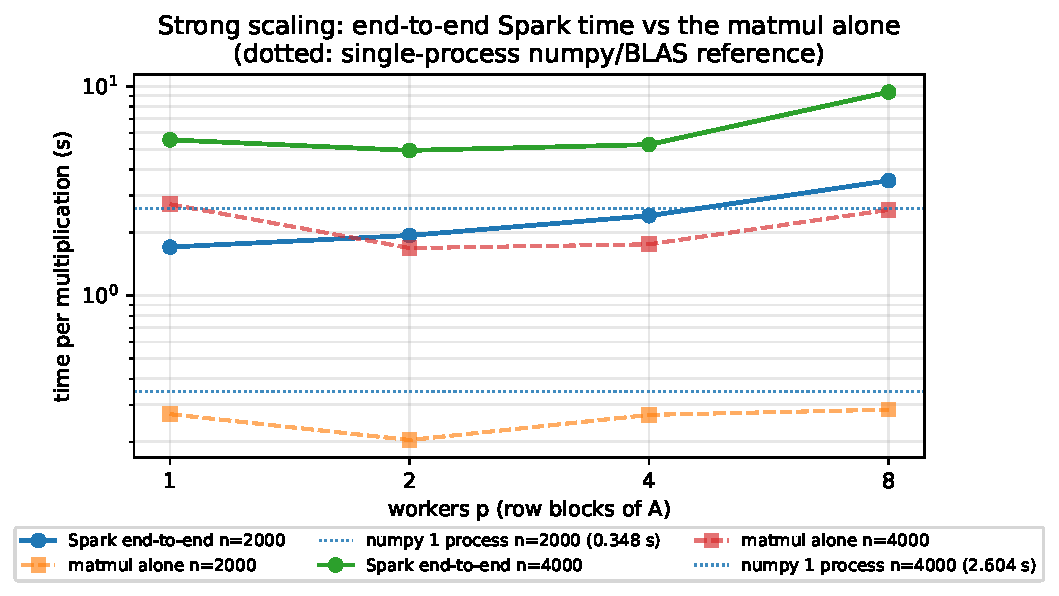
\includegraphics[width=0.9\textwidth]{fig1_strong.pdf}
\caption{Strong scaling at both problem sizes: end-to-end time and
multiplication-only time against the worker count, with the
single-process numpy/BLAS reference shown as dotted lines.}
\label{fig:strong}
\end{figure}

\begin{figure}[h!]
\centering
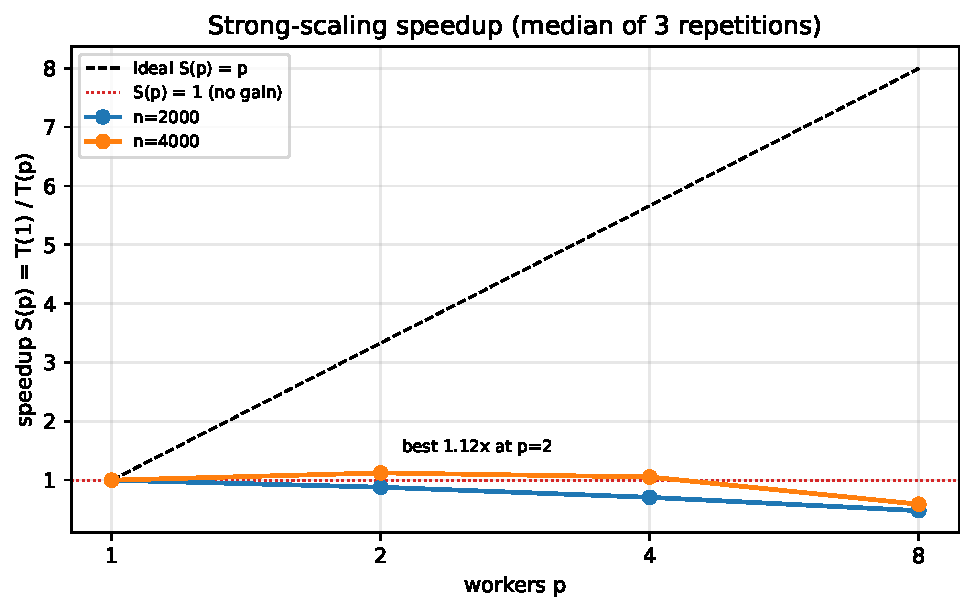
\includegraphics[width=0.78\textwidth]{fig2_speedup.pdf}
\caption{Strong-scaling speedup $S(p)=T_1/T_p$ against the ideal
$S(p)=p$; the dotted line at $S=1$ marks no gain. The best point is
$S=1.12$ at $p=2$ for $n=4000$.}
\label{fig:speedup}
\end{figure}

Scaling is \textbf{negative} almost everywhere. At $n=2000$ every
additional worker makes the multiplication slower: $T_8/T_1 = 2.08$. At
$n=4000$ there is a small gain at $p=2$ ($S=1.12$) which is erased at
$p=4$ and reversed at $p=8$ ($S=0.59$). Efficiency falls to $0.06$--$0.07$
at $p=8$. The reason is visible in the same table: the share of
$t_{e2e}$ spent multiplying is only 8--16\,\% at $n=2000$ and 27--53\,\%
at $n=4000$; the rest is overhead, and that overhead grows with $p$.

The variability of these medians is moderate: across the 16 distributed
configurations the median coefficient of variation is $4.6$\,\% (max
$10.9$\,\%).

\subsection{Where the time goes}

\begin{table}[h!]
\centering
\small
\setlength{\tabcolsep}{4pt}
\begin{tabular}{rr|rrrr|rr}
\toprule
 & & \multicolumn{4}{c|}{per repetition (s)} & \multicolumn{2}{c}{one-time
 (s)} \\
$n$ & $p$ & $t_{stage\_a}$ & $t_{action\_job}$ & $t_{assemble}$ &
$t_{e2e}$ & $t_{startup}$ & $t_{replicate}$ \\
\midrule
2000 & 1 & 0.053 & 1.644 & 0.007 & 1.703 &  8.96 & 2.12 \\
2000 & 2 & 0.061 & 2.061 & 0.008 & 1.935 & 11.82 & 2.47 \\
2000 & 4 & 0.064 & 2.383 & 0.007 & 2.404 & 14.27 & 2.88 \\
2000 & 8 & 0.061 & 3.621 & 0.010 & 3.536 & 17.44 & 6.17 \\
4000 & 1 & 0.377 & 5.941 & 0.025 & 5.544 & 11.71 & 3.71 \\
4000 & 2 & 0.283 & 4.463 & 0.025 & 4.934 & 11.83 & 2.75 \\
4000 & 4 & 0.238 & 4.807 & 0.033 & 5.260 & 13.47 & 2.94 \\
4000 & 8 & 0.248 & 9.114 & 0.049 & 9.378 & 13.32 & 8.58 \\
\bottomrule
\end{tabular}
\caption{Additive per-repetition decomposition of $t_{e2e}$ (the three
left columns sum to the fourth) and the one-time application costs
reported beside it.}
\label{tab:phases}
\end{table}

\begin{figure}[h!]
\centering
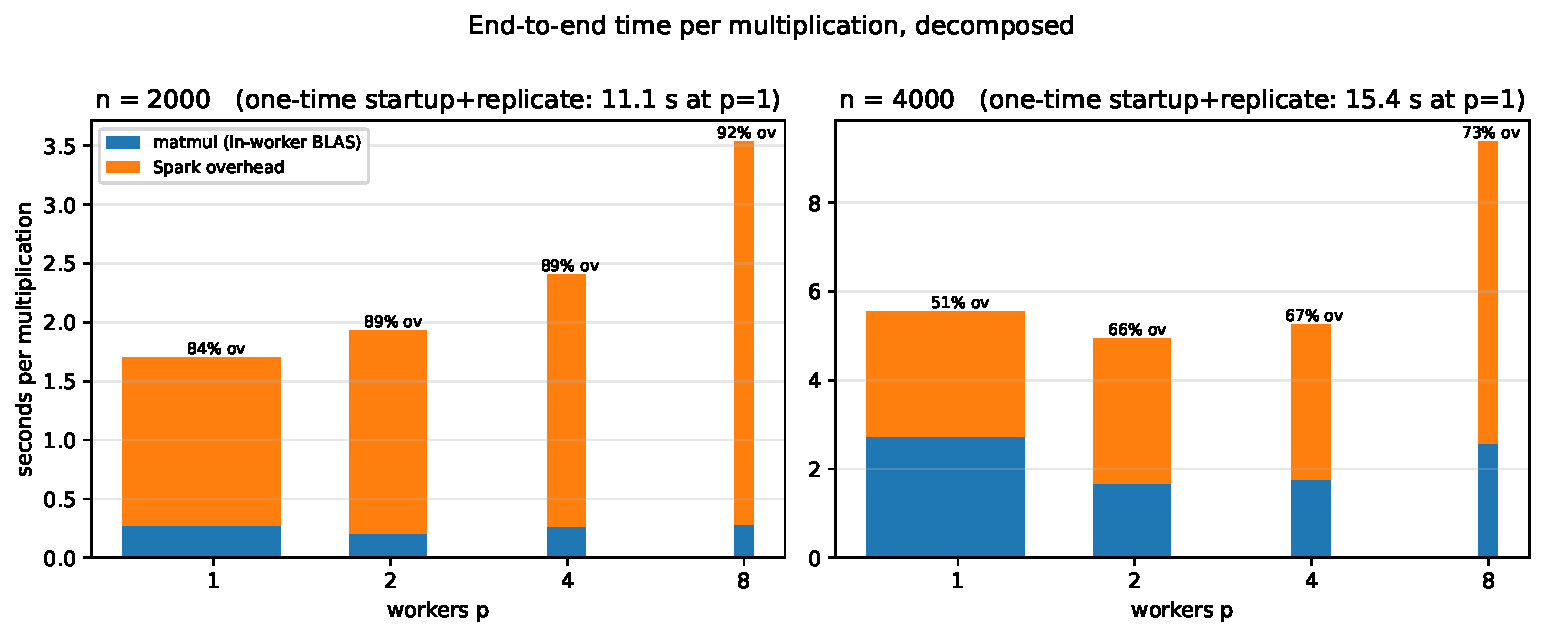
\includegraphics[width=0.9\textwidth]{fig5_overhead.pdf}
\caption{Composition of $t_{e2e}$: framework overhead against actual
multiplication, for both sizes and all worker counts. Start-up and
replication are one-time and are shown in the panel title, not stacked.}
\label{fig:overhead}
\end{figure}

$t_{assemble}$ is negligible (0.007--0.049\,s) and $t_{stage\_a}$ is small
but not free (0.05--0.38\,s, larger at $n=4000$ because serialising
$16$--$128$\,MB of row blocks is real driver work). Almost the whole
per-repetition cost sits in $t_{action\_job}$, and the one-time costs are
comparable to or larger than a whole repetition: starting the
application takes 9--17\,s and replicating $B$ takes 2--9\,s. At
$n=4000$, $p=8$, replicating $1.02$\,GB takes 8.58\,s, i.e.\ an
effective $\approx$119\,MB/s including the forcing job --- a loopback
transfer plus a Spark job, not a network measurement.

The event log localises the cost inside $t_{action\_job}$
(Table~\ref{tab:task}). On the critical path the worker spends far more
time getting ready to multiply than multiplying.

\begin{table}[h!]
\centering
\small
\setlength{\tabcolsep}{5pt}
\begin{tabular}{rrrrr}
\toprule
$n$ & $p$ & max task span (ms) & max task deserialisation (ms) &
max BLAS call (ms) \\
\midrule
2000 & 1 &  1706 &  594 &  271 \\
2000 & 8 &  6451 & 2616 &  284 \\
4000 & 1 &  6844 & 1399 & 2728 \\
4000 & 8 & 10661 & 4208 & 2568 \\
\bottomrule
\end{tabular}
\caption{Critical-path metrics from the Spark event log. The three
columns are maxima over tasks of the same run and are not necessarily
attained by the same task; they are sequential within a task and are
shown to locate the cost, not to be summed into $t_{e2e}$.}
\label{tab:task}
\end{table}

At $n=2000$, $p=8$, the slowest task spans 6.5\,s of which at most
0.28\,s is BLAS. At $n=4000$, $p=8$, deserialisation alone reaches
4.2\,s for a block of $16$\,MB, and the executor's run time reaches
8.0\,s against a 2.6\,s BLAS call. The gap is the cost of starting a
fresh Python worker for every task (see Section~\ref{sec:discussion}).

\subsection{Weak scaling}

The workload is grown as $n(p) = 2000 \cdot p^{1/3}$, rounded to
$\{2000, 2500, 3200, 4000\}$, which keeps $n^3/p$ at
$7.8$--$8.2 \times 10^9$ flop per worker (Table~\ref{tab:weak},
Figure~\ref{fig:weak}).

\begin{table}[h!]
\centering
\small
\setlength{\tabcolsep}{5pt}
\begin{tabular}{rrrrrrrr}
\toprule
$p$ & $n$ & $n^3/p$ & $t_{e2e}$ (s) & $T_p/T_1$ & weak eff. &
multiplication (s) & overhead \\
\midrule
1 & 2000 & $8.00\times10^9$ & 2.086 & 1.000 & 1.000 & 0.308 & 85.2\,\% \\
2 & 2500 & $7.81\times10^9$ & 2.261 & 1.084 & 0.922 & 0.381 & 83.2\,\% \\
4 & 3200 & $8.19\times10^9$ & 3.543 & 1.698 & 0.589 & 1.040 & 70.6\,\% \\
8 & 4000 & $8.00\times10^9$ & 7.747 & 3.714 & 0.269 & 1.940 & 75.0\,\% \\
\bottomrule
\end{tabular}
\caption{Weak scaling with constant work per worker $n^3/p$. Weak
efficiency is $T_1/T_p$.}
\label{tab:weak}
\end{table}

\begin{figure}[h!]
\centering
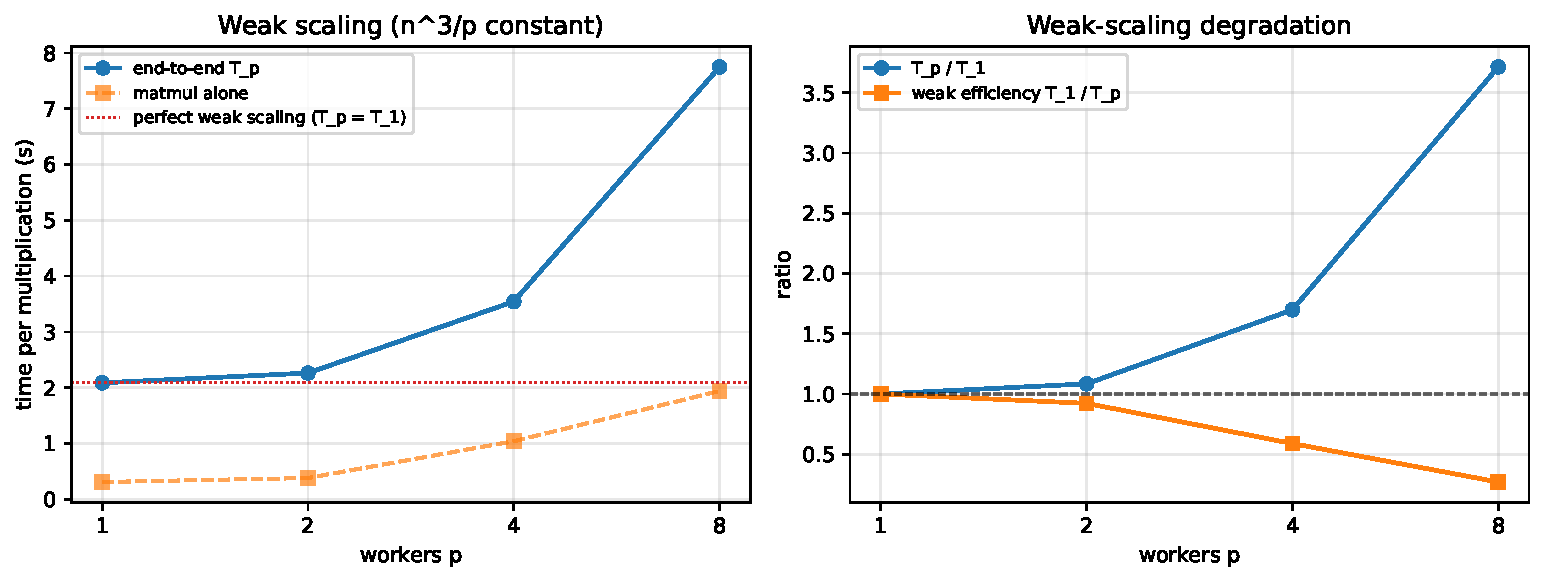
\includegraphics[width=0.95\textwidth]{fig3_weak.pdf}
\caption{Weak scaling at constant $n^3/p$: end-to-end time against the
ideal flat line (left) and the degradation ratio with weak efficiency
(right).}
\label{fig:weak}
\end{figure}

Weak efficiency falls from $0.92$ at $p=2$ to $0.27$ at $p=8$, i.e. the
same multiplication with eight times the resources per worker takes
$3.71\times$ longer in total. This is H4 confirmed: equal work per
worker does not give equal time, because start-up ($8.3 \rightarrow
22.2$\,s), replication ($2.4 \rightarrow 3.2$\,s) and the per-task
overheads all grow with $p$, while the multiplication itself grows only
$6.3\times$ for a $8\times$ larger operand (the local block is $p$ times
bigger, so the critical BLAS call grows from 0.31\,s to 1.94\,s).

\subsection{Size sweep}

Holding $p=4$ and varying $n$ isolates the fixed cost
(Table~\ref{tab:size}, Figure~\ref{fig:size}).

\begin{table}[h!]
\centering
\small
\setlength{\tabcolsep}{5pt}
\begin{tabular}{rrrrrr}
\toprule
$n$ & $t_{e2e}$ (s) & multiplication (s) & share & overhead &
$t_{startup}$ (s) \\
\midrule
 500 & 1.841 & 0.005 &  0.3\,\% & 99.7\,\% & 13.11 \\
1000 & 1.934 & 0.018 &  0.9\,\% & 99.1\,\% & 13.90 \\
2000 & 2.652 & 0.195 &  7.4\,\% & 92.6\,\% & 12.78 \\
4000 & 5.145 & 1.753 & 34.1\,\% & 65.9\,\% & 12.72 \\
\bottomrule
\end{tabular}
\caption{Size sweep at $p=4$. The end-to-end time has a floor of
$\approx$1.84\,s that is independent of $n$.}
\label{tab:size}
\end{table}

\begin{figure}[h!]
\centering
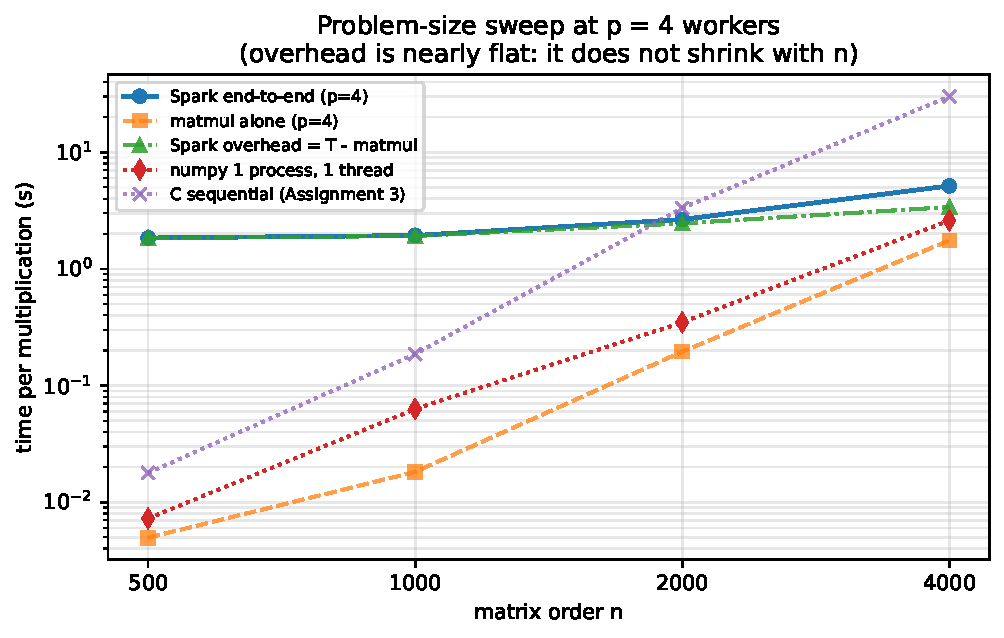
\includegraphics[width=0.82\textwidth]{fig4_size.pdf}
\caption{Size sweep at $p=4$: end-to-end time against matrix size, with
the multiplication-only time, the overhead (end-to-end minus
multiplication), and the single-process numpy/BLAS and Assignment~3
sequential C references for scale. The gap at small $n$ is the framework
floor.}
\label{fig:size}
\end{figure}

The end-to-end time starts at 1.84\,s for $n=500$ and only reaches
5.15\,s at $n=4000$: between $n=500$ and $n=1000$ the multiplication
grows $3.7\times$ (5\,ms $\rightarrow$ 18\,ms) while $t_{e2e}$ grows
only 5\,\%. The fixed per-repetition floor of $\approx$1.84\,s is
measured directly here, and it is what makes H1 true at every size
below $n=4000$.

\subsection{Comparison with the sequential and parallel baselines}

Three baselines run on the same inputs: the same numpy/BLAS kernel in
one process with one thread (the like-for-like reference that isolates
distribution cost), the Assignment~3 sequential C kernel, and the
Assignment~3 OpenMP/SIMD C kernel at 1, 2, 4 and 8 threads
(Table~\ref{tab:compare}, Figure~\ref{fig:compare}).

\begin{table}[h!]
\centering
\small
\setlength{\tabcolsep}{4pt}
\begin{tabular}{lrr|lrr}
\toprule
 & \multicolumn{2}{c|}{$n=2000$ (s)} & & \multicolumn{2}{c}{$n=4000$ (s)} \\
Implementation & time & vs.\ numpy & Implementation & time & vs.\ numpy \\
\midrule
numpy BLAS, 1 thread   & 0.348 & 1.00 & numpy BLAS, 1 thread   & 2.604 & 1.00 \\
C sequential           & 3.321 & 0.10 & C sequential           & 30.071 & 0.09 \\
C OpenMP, 8 threads    & 1.253 & 0.28 & C OpenMP, 8 threads    & 16.315 & 0.16 \\
\textbf{Spark, 1 worker}   & \textbf{1.703} & 0.20 & \textbf{Spark, 2 workers}
    & \textbf{4.934} & 0.53 \\
Spark, 2 workers       & 1.935 & 0.18 & Spark, 1 worker        & 5.544 & 0.47 \\
Spark, 4 workers       & 2.404 & 0.14 & Spark, 4 workers       & 5.260 & 0.49 \\
Spark, 8 workers       & 3.536 & 0.10 & Spark, 8 workers       & 9.378 & 0.28 \\
\bottomrule
\end{tabular}
\caption{Median end-to-end times. ``vs.\ numpy'' is the ratio to the
single-process, single-thread BLAS baseline; the best distributed
configuration at each $n$ is in bold.}
\label{tab:compare}
\end{table}

\begin{figure}[h!]
\centering
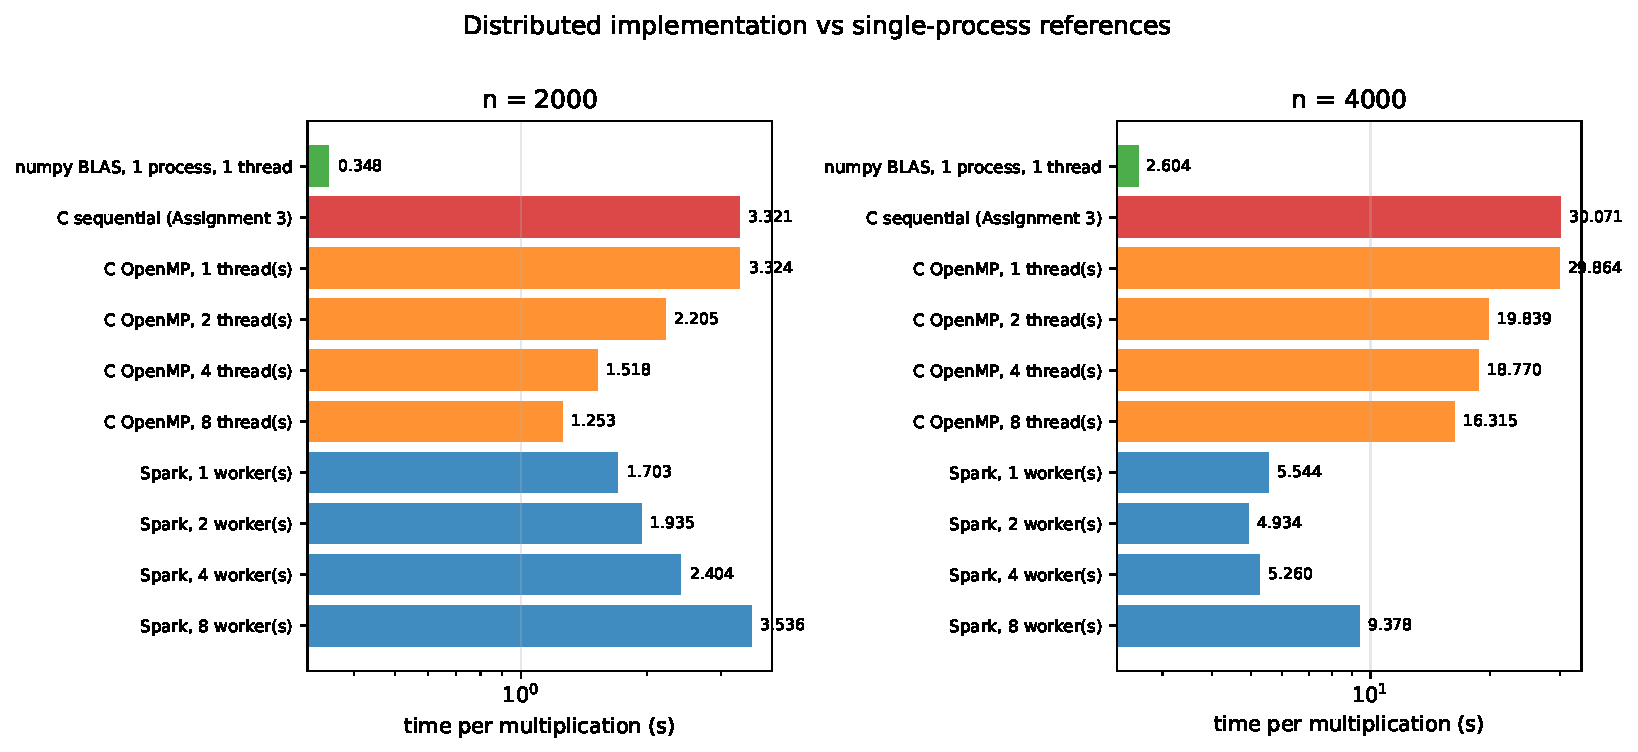
\includegraphics[width=0.9\textwidth]{fig6_compare.pdf}
\caption{All implementations at $n=2000$ and $n=4000$ on a logarithmic
axis. The distributed runs are compared with both the BLAS baseline and
the C kernels.}
\label{fig:compare}
\end{figure}

Against the like-for-like BLAS baseline (H3) the distributed version
loses everywhere: the best distributed run is $4.89\times$ slower at
$n=2000$ ($p=1$) and $1.89\times$ slower at $n=4000$ ($p=2$). Against
the \emph{C} baselines the picture differs by size, and this difference
is a kernel difference, not a distribution gain: at $n=2000$ the best
distributed run (1.703\,s) is still $1.36\times$ slower than the
8-thread OpenMP C kernel (1.253\,s), while at $n=4000$ it is
$3.31\times$ \emph{faster} than that same OpenMP kernel (4.934\,s vs.\
16.315\,s) because numpy's BLAS is several times faster than our
hand-written \texttt{ikj} kernel. Reporting either comparison alone
would be misleading, so both are given together with the kernel
difference stated.

An isolated comparison is prevented by three documented differences: the
distributed code uses a BLAS kernel while the C baselines use the
Assignment~3 scalar/OMP kernel; the distributed time is end-to-end
(driver phases included) while the C bench times are kernel-only; and
the distributed runs use a JVM framework while the C runs do not. These
differences are reported rather than removed.

\section{Discussion}
\label{sec:discussion}

\textbf{Answer to the research question.}
On this machine the distributed implementation does not scale: strong
scaling is negative beyond $p=2$, weak efficiency falls to $0.27$, and
the like-for-like comparison against single-process BLAS is lost by
$1.9$--$4.9\times$. The distribution itself is not the problem --- there
is no shuffle and the operand replication happens once per application
--- the problem is that a fixed framework cost of about $1.84$\,s per
repetition is paid on top of a multiplication that, at these sizes, takes
between 5\,ms and 2.7\,s.

Three causes, all quantified:

\begin{enumerate}
  \item \textbf{A per-repetition framework floor.} Measured directly by
        the size sweep: $t_{e2e}$ never drops below 1.84\,s at $p=4$
        (Figure~\ref{fig:size}), while the multiplication contributes
        0.3\,\% of it at $n=500$. This alone caps $S(p)$ well below 1
        for any $n$ whose multiplication is shorter than a few seconds.
  \item \textbf{Windows cannot reuse Python workers.}
        \texttt{PythonWorkerFactory.releaseWorker} only requeues a
        worker when \texttt{useDaemon} is true, and daemonisation needs
        \texttt{os.fork()}, which Windows does not provide. Every task
        therefore pays a fresh \texttt{python.exe}, the
        \texttt{import pyspark.worker} and the numpy import, on top of
        deserialising the row block. This is why the maximum task
        deserialization reaches 4.2\,s and the maximum executor run
        time 8.0\,s for 2.6\,s of BLAS at $n=4000$, $p=8$
        (Table~\ref{tab:task}), and why $t_{action\_job}$ grows with $p$
        even though the blocks shrink. It is framework overhead, in
        scope for this assignment, but it is a platform artifact rather
        than an inherent property of the algorithm.
  \item \textbf{The hardware caps useful parallelism.}
        On the same BLAS kernel and the same inputs, one thread delivers
        65.1\,GFLOP/s and eight threads 121.3\,GFLOP/s --- only
        $1.86\times$ --- because the i7-1355U is a 15\,W part with two
        performance cores and eight efficiency cores. Eight workers
        cannot be $8\times$ faster than one even with free
        communication, so any scaling study on this machine has a
        ceiling of about $1.9\times$ before framework costs are counted.
\end{enumerate}

\textbf{On the negative strong-scaling result.}
It is a valid measurement, not a bug: the event log confirms
\texttt{peak\_concurrent\_tasks} $= p$ for every configuration, all 20
validated outputs satisfy $\textit{allclose}$ against the sequential C
reference (maximum absolute difference $6.96\times10^{-13}$), and
shuffle traffic is exactly zero. The work is genuinely concurrent; it is
simply dwarfed by costs that grow with $p$.

\textbf{What would be needed to see positive scaling.}
Two things, in order: make the per-repetition floor much smaller than
the multiplication (larger $n$, or an amortised/multiplied application),
and remove the per-task process spawn (a platform with daemon-capable
workers, or a JVM-side kernel). The first is available on this machine
only up to $n=4000$, where the multiplication still reaches just 34\,\%
of $t_{e2e}$.

\section{Limitations}

\begin{itemize}
  \item \textbf{Local execution only.} All workers are processes on one
        physical laptop over loopback. No physical network, no
        inter-node transfer and no multi-machine memory capacity are
        exercised or claimed; network cost cannot be isolated because
        there is no network to isolate it from.
  \item \textbf{Small cluster, small inputs.} $p \le 8$ workers of one
        core and $n \le 4000$ ($128$\,MB per matrix). Inputs larger than
        one machine's memory were not attempted; with 16.8\,GB available
        they would not have been meaningful anyway.
  \item \textbf{No process-level memory measurement.} Per-worker memory
        is reported as block-manager capacity from the event log;
        resident set size of the worker JVMs and of the Python workers
        was not sampled, so peak physical memory per worker is unknown.
  \item \textbf{Platform artifacts dominate.} The Windows
        worker-respawn behaviour inflates $t_{action\_job}$ and is not
        representative of a POSIX deployment; results here characterise
        this configuration, not Spark in general.
  \item \textbf{One outlier retained.} One baseline repetition
        (\texttt{c\_omp}, $n=4000$, 8 threads) recorded 773.6\,s against
        a 16.3\,s median, evidently a machine stall. The median is
        reported and the raw value is left in the CSV for transparency.
  \item \textbf{No hardware counters.} Windows offers no usable
        performance-counter access here, so the split between
        deserialization, process start and transfer inside a task is
        taken from Spark's own event-log timers only.
  \item \textbf{One machine, one input distribution.} As in
        Assignments~1--3, claims are limited to these implementations,
        inputs and hardware~\cite{fleming1986,mytkowicz2009}.
\end{itemize}

\section{Conclusions}

Within the tested scope:
\begin{enumerate}
  \item The row-block design with a replicated operand is correct and
        shuffle-free: 20/20 validated configurations pass with maximum
        absolute difference $6.96\times10^{-13}$, and all 40
        configurations complete successfully.
  \item Strong scaling is negative. At $n=2000$ the time rises from
        1.703\,s ($p=1$) to 3.536\,s ($p=8$), $S(8)=0.48$; at $n=4000$
        the best point is $S(2)=1.12$ and $S(8)=0.59$. Efficiency never
        exceeds $0.57$ except at the trivial $p=1$ reference.
  \item Between 51\,\% and 92\,\% of the end-to-end time is framework
        overhead, and the overhead share \emph{rises} with $p$. A fixed
        floor of $\approx$1.84\,s per repetition is measured directly at
        $p=4$.
  \item Weak scaling degrades to weak efficiency $0.27$ at $p=8$
        ($T_8/T_1 = 3.71$) despite constant work per worker of
        $\approx 8\times10^9$ flop.
  \item Against the like-for-like single-process BLAS baseline the
        distributed run is $4.89\times$ slower at $n=2000$ and
        $1.89\times$ slower at $n=4000$; against the Assignment~3 C
        baselines it is $1.36\times$ slower at $n=2000$ and
        $3.31\times$ faster at $n=4000$, the latter being a BLAS-versus-
        hand-written-kernel difference rather than a distribution gain.
  \item Start-up (9--17\,s) and operand replication (2--9\,s) are
        one-time but large, and must be reported beside $t_{e2e}$ rather
        than folded into it.
  \item Three causes dominate and are measured: the framework floor,
        per-task Python-worker respawn on Windows (up to 4.2\,s of
        deserialization for a 16\,MB block), and a CPU whose BLAS
        throughput saturates at $1.86\times$ from one to eight threads.
\end{enumerate}

Open questions: how much of the floor disappears on a POSIX deployment
with reusable workers, whether an amortised application that performs
many multiplications per start-up changes the sign of the scaling, and
how the same design behaves with $p$ larger than the core count.

\section{References and materials}

{\sloppy
All source code (\texttt{src/spark/distributed\_matmul.py},
\texttt{src/spark/sparkconf.py}, \texttt{scripts/run\_benchmark4.py},
\texttt{scripts/spark\_cluster.py}, \texttt{scripts/collect\_env.py}),
the shared inputs, the framework configuration, raw measurements
(\texttt{configs4.csv}, \texttt{raw\_timings4.csv}, JSON lines per run
in \texttt{data/results/raw\_detail/}), \texttt{environment.json}, the
executed analysis notebook and every figure are in the public repository
\url{https://github.com/aledelgadoo/individual-assignments-bigdata}.
The Git tag \texttt{assignment-4} marks the submitted state; tags
\texttt{assignment-1}, \texttt{assignment-2} and \texttt{assignment-3}
keep the earlier work. \texttt{README.md} documents the environment,
cluster, campaign and analysis commands that regenerate this report end
to end, and \texttt{notebooks/04\_analysis.ipynb} writes the summary
tables (\texttt{summary\_strong.csv}, \texttt{summary\_weak.csv},
\texttt{summary\_size.csv}, \texttt{summary\_compare.csv}) quoted here.\par}

\section*{Generative-AI usage statement}

Following the course policy, the author discloses that the AI assistant
\textbf{opencode} (model \texttt{opencode/mimo-v2.6-flash-free}) was
used, under the author's direction, for planning the PySpark design and
the measurement protocol, drafting and debugging the Python code and
the benchmark harness, diagnosing the Windows \texttt{sc.broadcast} and
Python-worker limitations, generating the analysis notebook and figures,
and revising the English of this report. The author reviewed all
generated code, supervised every campaign execution and the pilot gate,
verified the numbers quoted here against the raw CSV and JSON-lines
files, and is responsible for the measurements, the conclusions and any
errors.

{\small
\begin{thebibliography}{9}
\bibitem{zaharia2012}
M. Zaharia, M. Chowdhury, T. Das, A. Dave, J. Ma, M. McCauley,
M. Franklin, S. Shenker, and I. Stoica, ``Resilient distributed datasets:
A fault-tolerant abstraction for in-memory cluster computing,'' in
\emph{Proc. 9th USENIX Conf. on Networked Systems Design and
Implementation (NSDI)}, 2012, pp. 15--28.

\bibitem{fleming1986}
W. P. Fleming and J. M. Wallace, ``How not to lie with statistics: the
correct way to summarize benchmark results,'' \emph{Communications of
the ACM}, vol. 29, no. 3, pp. 218--221, 1986.

\bibitem{mytkowicz2009}
T. Mytkowicz, A. Diwan, M. W. Hauswirth, and P. F. Sweeney,
\emph{Measuring Computer Performance: A Practitioner's Guide}.
Cambridge University Press, 2009.

\bibitem{sparkdoc}
Apache Software Foundation, \emph{Apache Spark 4.3 Documentation:
Standalone Mode, Broadcast Variables, and Python Workers}. [Online].
Available: \url{https://spark.apache.org/docs/4.3.0/}

\bibitem{numpy}
C. R. Harris \emph{et al.}, ``Array programming with numpy,''
\emph{Nature}, vol. 585, pp. 357--362, 2020.

\bibitem{strang2016}
G. Strang, \emph{Introduction to Linear Algebra}, 5th ed.
Wellesley--Cambridge Press, 2016.

\bibitem{psutil}
G. Rodola, \emph{psutil: cross-platform process and system utilities},
2026. [Online]. Available: \url{https://github.com/giampaolo/psutil}
\end{thebibliography}}

\end{document}
